\documentclass[USenglish,oneside,twocolumn]{article}

\usepackage[utf8]{inputenc}
\usepackage[big]{dgruyter_NEW}
\usepackage[T1]{fontenc}
\usepackage[scaled=0.8]{beramono}
\usepackage[defaultsans,scale=0.9]{cantarell}
\usepackage[linesnumbered,boxed]{algorithm2e}
\usepackage{tikz}
\usepackage{amsmath}
\usepackage[mark,raisemark=-1cm]{gitinfo2}

\definecolor{darkblue}{rgb}{0,0,0.7}
\hypersetup{
	colorlinks=true,
	urlcolor=darkblue,
	linkcolor=darkblue,
	citecolor=darkblue
}

\urlstyle{sf}

\renewcommand*{\bibfont}{\small}
\newcommand{\mynote}[1]{\noindent\textcolor{red}{\textbf{Note:} #1}}

\cclogo{
\includegraphics{by-nc-nd.pdf}}

\begin{document}

\author{Anonymous}

\title{\huge Identifying and characterizing\\Sybils in the Tor network}

\runningtitle{Identifying and characterizing Sybils in the Tor network}

\subsection*{Abstract}
Being a volunteer-run, distributed anonymity network, Tor is vulnerable to Sybil
attacks.  Little is known about real-world Sybils in the Tor network, and we
lack practical tools and methods to expose Sybil attacks.
%
In this work, we develop \sys, the first system for detecting Sybil relays based
on their \emph{appearance}, such as configuration; and \emph{behavior}, such as
uptime sequences.  We used \sys's diverse analysis techniques to analyze nine
years of archived Tor network data, providing us with new insights into the
operation of real-world attackers.  Our findings include diverse incidents,
ranging from botnets, to academic research, and relays that hijack Bitcoin
transaction.
%
Our work shows that existing Sybil defenses do not apply to Tor, it delivers
insights into real-world attacks, and provides practical tools to expose and
characterize Tor relays, making the network safer for its users.


\keywords{Tor, Sybil attack}

\journalname{Proceedings on Privacy Enhancing Technologies}
\DOI{Editor to enter DOI}
\startpage{1}
\received{..}
\revised{..}
\accepted{..}

\journalyear{2015}
\journalvolume{2015}
\journalissue{2}

\maketitle

\section{Introduction}
\label{sec:introduction}

% Short introduction to Sybil attacks.
In a Sybil attack, an attacker controls many virtual identities to
obtain disproportionately large influence in a network.  These attacks take many
shapes, such as sockpuppets hijacking online discourse~\cite{Thomas2012a}; the
manipulation of BitTorrent's distributed hash table~\cite{Wang2012a}; and, most
relevant to our work, relays in the Tor network that seek to deanonymize
users~\cite{cmucert}.  Preventing Sybil attacks remains challenging, as
evidenced by Douceur's seminal 2002 paper that shows that Sybil attacks are
always possible in the absence of a central authority~\cite{Douceur2002a}.  In
this work, we focus on Sybils in the Tor network, i.e., Tor relays (virtual
identities) that are controlled by a single operator (physical entity).  But
what harm can Sybils do in Tor?

The effectiveness of many attacks on Tor depends on how large a fraction of the
network's traffic---the consensus weight---an attacker can observe.  As the
attacker's consensus weight grows, she is increasingly able to launch attacks
such as:
\begin{description}
	\item[Exit traffic tampering:] A Tor user's traffic traverses exit relays, the
		last hop in a Tor circuit, when leaving the Tor network.  Having control
		over exit relays, an attacker can sniff traffic to harvest unencrypted
		credentials, break into TLS-protected connections, or inject traffic
		such as advertisements~\cite{Winter2014a}.
	\item[Website fingerprinting:] Tor's encryption prevents guard relays (the
		first hop in a Tor circuit) from learning their user's online activity.
		Ignoring the encrypted payload, an attacker can still take advantage of
		flow information such as packet lengths and timings to infer what web
		site its users are connecting to~\cite{Juarez2014a}.
	\item[Bridge address harvesting:] Users behind censorship firewalls use
		bridges---basically non-public Tor relays---as hidden stepping stones
		into the Tor network.  It is important that censors cannot obtain all bridge
		addresses, which is why bridge distribution is rate-limited.  An
		attacker can harvest bridge addresses by running a middle relay and
		looking for incoming connections that do not originate from guard
		relays.  These have to be bridge addresses~\cite{Ling2012a}.
	\item[End-to-end correlation:] By running both entry guards and exit relays,
		the attacker can use timing analysis to link a Tor user's activity to
		her identity, e.g., learn that Alice visited Facebook.  For this attack,
		an attacker must run at least two Tor relays~\cite{Johnson2013a}.
\end{description}

% Scale horizontally when we run out of consensus weight.
An attacker can increase its consensus weight by configuring her relay to
forward more traffic.  However, the capacity of a single relay is limited by its
link bandwidth and, because of the computational cost of cryptography, by CPU.
Once an adversary reaches this limit, she has to scale horizontally, i.e., add
more Sybil relays to the network.

% Sybils are needed to manipulate the DHT, and can be a side effect.
Besides the above attacks, an adversary needs Sybil relays to manipulate onion
services, which are TCP servers whose IP address is hidden by Tor.  Six Sybil
relays are sufficient to take offline an onion service because of a weakness in
the design of the distributed hash table (DHT) that powers onion
services~\cite{Biryukov2013a}.  Finally, instead of being a direct means to an
end, Sybil relays can be a \emph{side effect} of another issue.  In
Section~\ref{sec:sybil_groups}, we provide evidence for what appears to be
botnets whose zombies are running Tor relays, perhaps because of a misguided
attempt to help the Tor network grow.  The zombie owners are likely unaware of
the relays they are running.

% Existing Sybil defense mechanisms.
Sybil attacks are a well-known problem to The Tor Project, which is reflected in
a number of both implicit and explicit Sybil defenses that are in place as of
Dec 2015.  First, directory authorities---the ``gatekeepers'' of the Tor
network---accept at most two relays per IP address~\cite{Bauer2007b} to prevent
low-resource Sybil attacks~\cite{Bauer2007a}.  Similarly, Tor's path selection
algorithm~\cite{path-spec} incorporates heuristics so Tor clients avoid relays
that could be controlled by the same operator, e.g., Tor clients never select
two relays in the same /16 network.  Second, directory authorities assign flags
to relays, indicating their status and quality of service.  The Tor Project has
recently increased the minimal time until relays obtain the \texttt{Stable} flag
(seven days) and the \texttt{HSDir} flag (96 hours).  This change increases the
cost of Sybil attacks and gives Tor developers more time to discover suspicious
relays before they get in a position to run an attack.  Finally, operating a Tor
relay causes recurring costs---most notably bandwidth and electricity---which
can further limit an adversary.

% Our contributions.
Motivated by the lack of practical Sybil detection tools, we design and
implement heuristics, leveraging that Sybils 1) frequently go online and offline
simultaneously, 2) share similarities in their configuration, and 3) may change
their identity fingerprint---a relay's fingerprint is the hash over its public
key---frequently, to manipulate Tor's DHT.  We implemented
these heuristics in a tool, sybilhunter, which we then use to analyze historical
network data, dating back to as early as 2007, to discover past attacks and
anomalies.  Finally, we characterize the Sybil groups we discover.  To sum up,
we make the following key contributions:
\begin{itemize}
	\item We design and implement a tool---sybilhunter---to analyze past and
		future Tor data.  Our approach does not require any modifications to the
		Tor network, finds similarities in relays' configuration and their
		uptime sequences.
	\item We expose and characterize Sybil groups and publish a dataset to
		stimulate future research.  We find that many different kinds of
		operators run Sybil groups, including financially-motiviated attackers,
		researchers, and unskilled troublemakers.
\end{itemize}

% Structure of the paper.
The rest of this paper is structured as follows.  We begin by discussing
related work in Section~\ref{sec:related_work}.  Section~\ref{sec:design}
presents the design of our analysis tools, which is then followed by
experimental results in Section~\ref{sec:results}.  We discuss our results in
Section~\ref{sec:discussion} and conclude the paper in
Section~\ref{sec:conclusion}.


\section{Related work}
\label{sec:related_work}
In his seminal 2002 paper, Douceur showed that only a \emph{central authority}
that verifies new nodes as they join the distributed system is guaranteed to
prevent Sybils~\cite{Douceur2002a}.  This approach conflicts with Tor's design
philosophy that seeks to distribute trust and eliminate central points of
control.  In addition, a major factor contributing to Tor's network growth is
the low barrier of entry, allowing operators to set up relays both quickly and
anonymously.  An identity-verifying authority would raise that barrier, alienate
privacy-conscious relay operators, and impede Tor's growth.  Barring a central
authority, researchers have proposed techniques that leverage a resource that is
difficult for an attacker to scale.  Two categories of Sybil-resistant schemes
turned out to be particularly popular, schemes that build on \emph{social
constraints} and schemes that build on \emph{computational constraints}.  For a
broad overview of alternative Sybil defenses, refer to Levine et
al.~\cite{Levine2006a}.

Social constraints rely on the assumption that it is difficult for an attacker
to form trust relationships with honest users, e.g., befriend many unknown
people on online social networks.  Past work leveraged this assumption in
systems such as SybilGuard~\cite{Yu2006a}, SybilLimit~\cite{Yu2008a}, and
SybilInfer~\cite{Danezis2009a}.  Unfortunately, social graph-based defenses
do not work in our setting because there is no existing trust relationship
between relay operators.\footnote{Relay operators can express in their
configuration that their relays are run by the same operator, but this
denotes an \emph{intra}-person and not an \emph{inter}-person trust
relationship.} Note that we could create such a relationship by, e.g., linking
relays to their operator's social networking account, or by creating a ``relay
operator web of trust,'' but again, we believe that such an effort would
alienate relay operators and receive limited adoption.

Orthogonal to social constraints, computational resource constraints guarantee
that an attacker that seeks to operate 100 Sybils needs 100 times the
computational resources she would have needed for a single virtual identity.
Both Borisov~\cite{Borisov2006a} and Li et al.~\cite{Li2012a} used computational
puzzles for that purpose.  Computational constraints work well in distributed
systems where the cost of joining the network is low.  For example, a
lightweight client is enough to use BitTorrent, allowing even low-end consumer
devices to participate.  However, this is not the case in Tor because relay
operations require constant use of bandwidth and CPU.  Unlike in many other
distributed systems, it is impossible to run 100 Tor relays while not spending
the resources for 100 relays.  Computational constraints are inherent to running
a relay.

In summary, we believe that existing Sybil defenses do not work well when
applied to the Tor network; its distinctive features call for customized
solutions that consider the nature of Tor relays.  There has already been
some progress towards that direction; namely, The Tor Project has incorporated
a number of both implicit and explicit Sybil defenses that are in place as of
February 2016.  First, directory authorities---the ``gatekeepers'' of the Tor
network---accept at most two relays per IP address to prevent low-resource Sybil
attacks~\cite{Bauer2007a,Bauer2007b}.  Similarly, Tor's path selection algorithm
states that Tor clients never select two relays in the same /16
network~\cite{path-spec}.  Second, directory authorities automatically assign
flags to relays, indicating their status and quality of service.  The Tor
Project has recently increased the minimal time until relays obtain the
\texttt{Stable} flag (seven days) and the \texttt{HSDir} flag (96 hours).  This
change increases the cost of Sybil attacks and gives Tor developers more time to
discover and block suspicious relays before they get in a position to run an
attack.  Finally, the operation of a Tor relay causes recurring costs---most
notably bandwidth and electricity---which can further restrain an adversary.


\section{Design}
\label{sec:design}
We now discuss the design philosophy behind sybilhunter, our Sybil detection
tool.  Sybilhunter takes as input archived Tor network data, and then attempts
to isolate Sybil groups.  The big picture is shown in Figure~\ref{fig:system}.
We motivate our design decisions with the experience we gained by manually
analyzing numerous Sybil groups in the Tor network.  We iteratively improved
and refactored sybilhunter when we experienced operational shortcomings.  We
further augment our design with ideas from related work, e.g., Cao et al.
observed that Sybil groups have things in common and changes happen more or
less at the same time~\cite{Cao2014a}.

\begin{figure}[t]
	\centering
	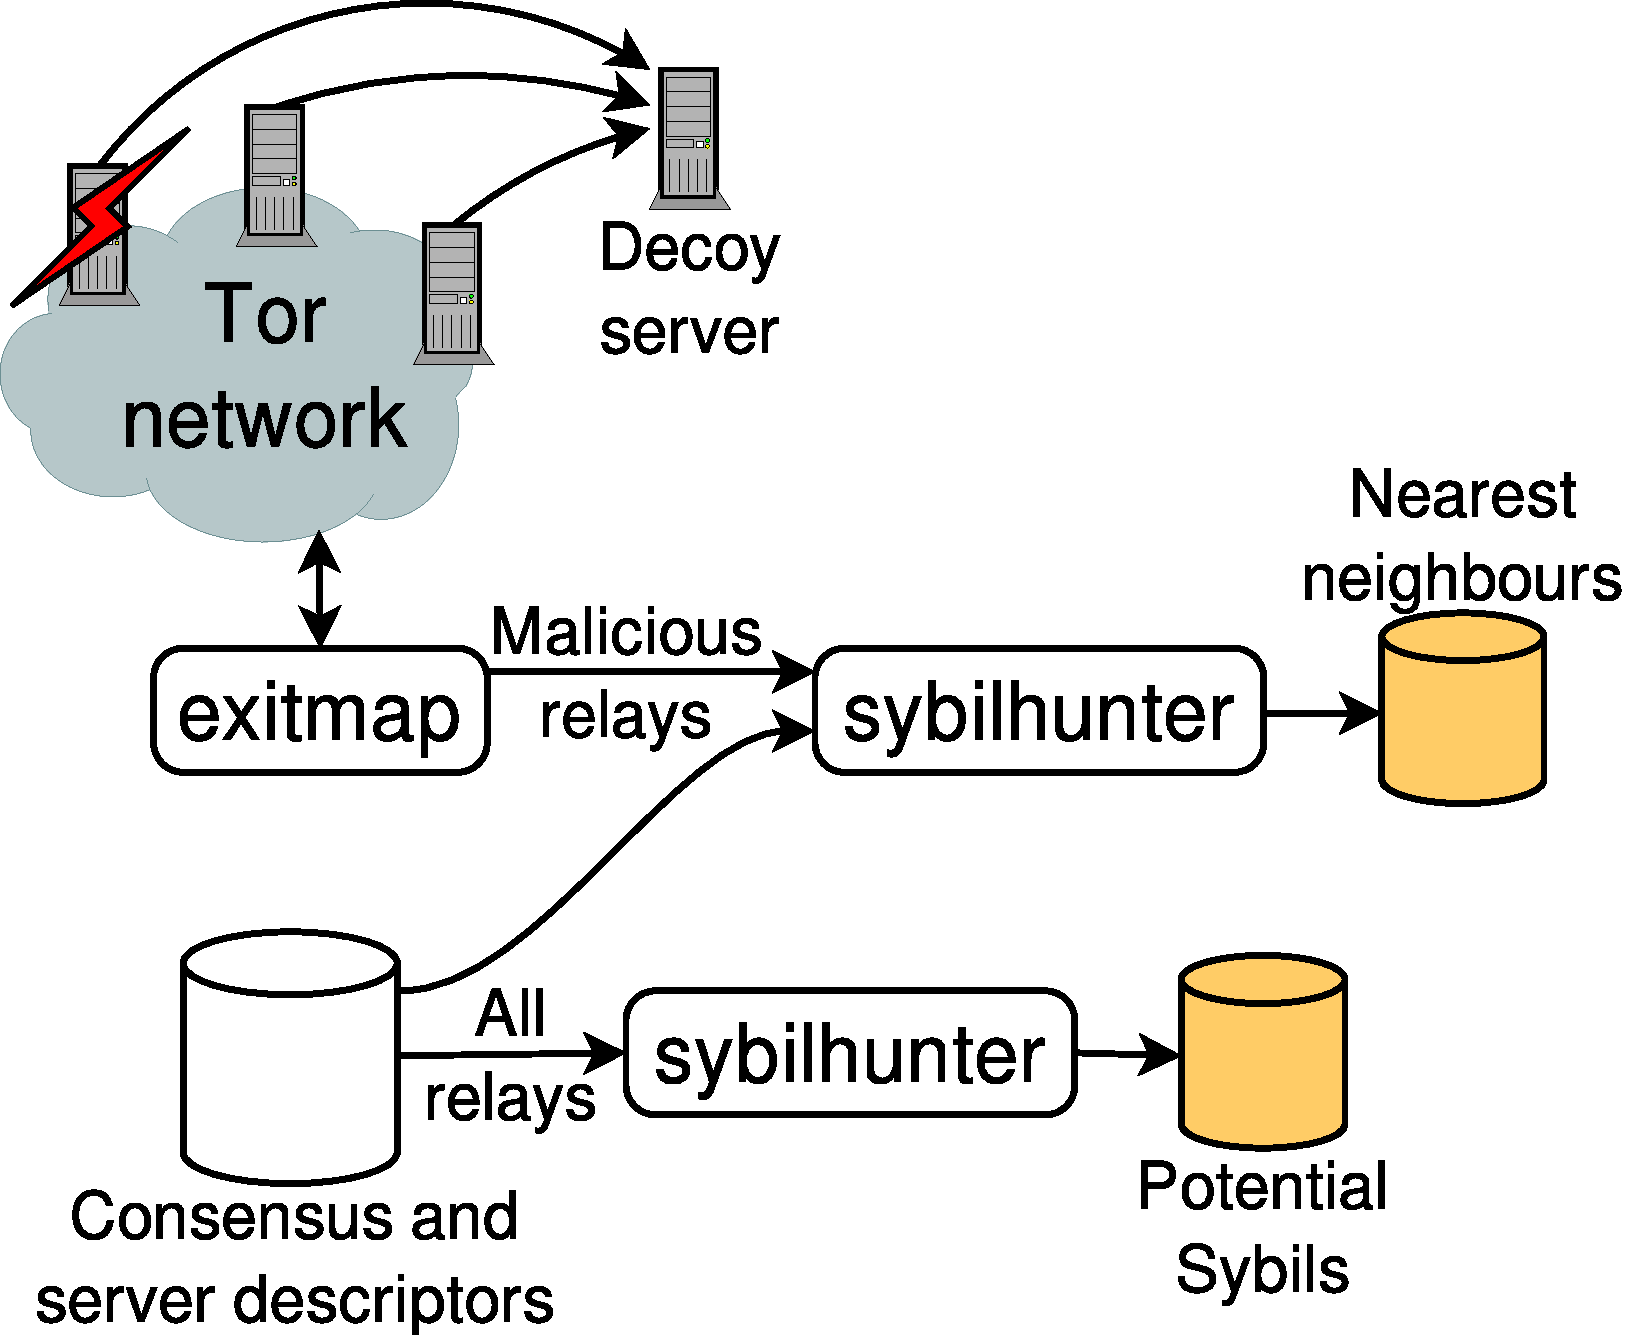
\includegraphics[width=0.42\textwidth]{diagrams/system_architecture.pdf}
	\caption{Our system architecture.  Two different data sets serve as input
		to sybilhunter, our Sybil detection tool; 1) archived consensuses and
		server descriptors, and 2) malicious relays that we gather by running
		exitmap~\cite{Winter2014a}.  Sybilhunter then attempts to extract Sybil
		groups from the given data.}
	\label{fig:system}
\end{figure}

Sybilhunter is designed to run in different scenarios.  We can 1) run it over
historical network data, ranging back to 2007, 2) run it online to detect new
Sybils as they join the network, and 3) use it to find relays that are
potentially associated with previously discovered bad exit relays.

Generally speaking, we seek to isolate relays that are similar in
\emph{appearance} (\S~\ref{sec:nearest-neighbor}) as well as in \emph{behavior}
(\S~\ref{sec:churn-time-series}, \S~\ref{sec:uptime-matrix}, and
\S~\ref{sec:fingerprint-analysis}).  The following sections discuss our data sets
and analysis modules of sybilhunter.

\mynote{Can we model the arrival rate of relay descriptor as Poisson process
and find outliers in it?}

\subsection{Data sets}
\label{sec:datasets}
We employ two types of data sets, both of which are illustrated in
Figure~\ref{fig:system}.  First, we mine \emph{archived consensuses and server
descriptors} for relay clusters and second, we use the \emph{output of the
exitmap scanner} (in combination with archived data) to find associated,
malicious relays.

\subsubsection{Consensuses and router descriptors}
We took the data sets we use for our analyses from CollecTor~\cite{collector},
a service run by The Tor Project that archives network data such as
consensuses, router descriptors, and network status votes.  Some of the
archived data dates back to as early as 2004, allowing us to restore arbitrary
Tor network states in the last ten years.  CollecTor archives numerous data
sources, but not all are relevant for our hunt for Sybils, which is why we only
analyse the following two:

\begin{description}
	\item[Descriptors] Tor relays and bridges periodically upload server
		descriptors, which capture their configuration, to directory
		authorities.  Relays upload their descriptors no later than every 18
		hours, or sooner, depending on certain conditions.

	\item[Consensuses] The Tor network's consensus contains a list of all
		running Tor relays.  Directory authorities vote hourly on the state of
		the network, and the outcome is the consensus.  Every relay status in
		the consensus contains a digest that is used to obtain the relay's
		respective descriptor, as can be seen in Figure~\ref{fig:datasets}.
\end{description}

\begin{figure}[t]
	\centering
	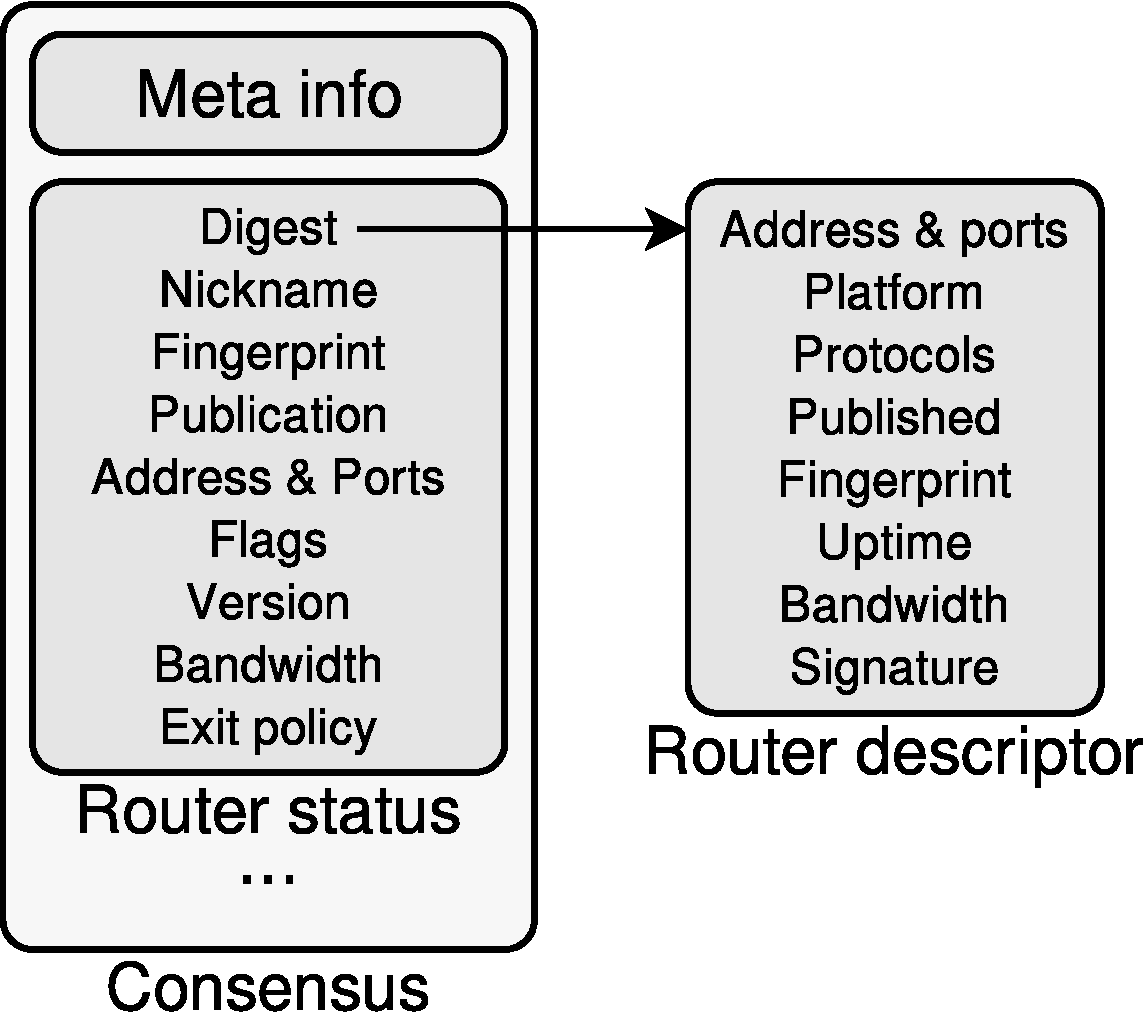
\includegraphics[width=0.3\textwidth]{diagrams/data_sets.pdf}
	\caption{Our data set contains consensuses and router descriptors.  This
		diagram shows how they relate to each other.}
	\label{fig:datasets}
\end{figure}

Table~\ref{tab:collector-dataset} gives an overview of the size of our data
sets.  We found it challenging to process such large amounts of data.  We
started by using the Python parsing library Stem, which is maintained by The Tor
Project.  The size of the data sets as well as the amount of files turned out to
be difficult to handle for Stem because it was implemented in an interpreted,
dynamic language.

\begin{table}[t]
\centering
\begin{tabular}{l c c c}
\textbf{Data set} & \textbf{Files} & \textbf{Size} & \textbf{Time span} \\
\hline
% 47677982862 bytes.
Consensuses & 67,671 & 44 GiB & 10/2007 -- 07/2015 \\
% 48252370463 bytes.
Descriptors & 30,759,243 & 44 GiB & 12/2005 -- 07/2015 \\
% 1375933490 bytes.
% Torperf data & 18,348 & 1 GiB & 07/2009 -- 07/2015 \\
\end{tabular}
\caption{Characterization of our data sets.}
\label{tab:collector-dataset}
\end{table}

\begin{table}[t]
\centering
\begin{tabular}{l c p{4cm}}
\textbf{Discovery} & \textbf{\# of relays} & \textbf{Incident} \\
\hline
% Message-ID: <20151117150055.GA25187@nymity.ch>
2015-11-17 & 8 & Downgrade TLS and replace onion domains. \\
% Message-ID: <20151116164403.GL10892@nymity.ch>
2015-11-16 & 1 & SSLStrip attack. \\
% Message-ID: <20150926174033.GB27610@nymity.ch>
2015-09-26 & 6 & Blocking STARTTLS over SMTP. \\
% Message-ID: <20150804202838.GA4774@nymity.ch>
2015-08-04 & 4 & Onion service impersonation by rewriting onion domains. \\
% Message-ID: <20150630022923.GA2340@nymity.ch>
2015-06-29 & 55 & Onion service impersonation by rewriting onion domains. \\
% Message-ID: <20150423004031.GA11395@nymity.ch>
2015-04-22 & 70 & Onion service impersonation by rewriting onion domains. \\
% Message-ID: <20150311125831.GD23215@nymity.ch>
2015-03-11 & 1 & Injected iframe into relayed HTML. \\
\end{tabular}
\caption{Characterization of the bad exit relays we collected.}
\label{tab:exitmap-dataset}
\end{table}

We then implemented a new parser from scratch in the Go programming
language~\cite{zoossh}.  Our parser consists of approximately 2,000 lines of
code (and 1,000 more lines for tests) and supports strict and lazy parsing, to
minimize unnecessary parsing.  According to our benchmarks, our parser is able
to parse approximately 27 consensuses per second.\footnote{Measured on an Intel
Core i7 2.9 GHz CPU.  We placed our data sets on a solid state drive to
minimize I/O.}  Stem, for comparison, averages at around 1.8 consensuses per
second.\footnote{Note, however, that Stem parses slightly more fields than our
parser, which means that both parsers would be closer together in a fair
comparison.}

Figure~\ref{fig:datasets} illustrates the relationship between our data.
Primarily, we are interested in the hourly consensus files.  A consensus file
consists of \emph{router statuses} that contain basic information about Tor
relays such as its bandwidth, flags, and exit policy.  As of August 2015,
consensuses contain approximately 6,000 router statuses.  Every router status
contains a digest that is used to locate its corresponding \emph{router
descriptor}.  It is important to understand that router descriptors are
published as they were received by Tor relays whereas consensus files are voted
on, and published, by directory authorities.  Some fields in a router status
are also subject to verification.  For example, the Tor network operates
bandwidth scanners that verify if a relay is able to sustain the bandwidth it
claims to handle in its router descriptor.

\subsubsection{Malicious relays}
We use a second, complementary data set that consists of malicious exit relays
we gather by running exitmap~\cite[\S 3.1]{Winter2014a}.  The dataset is shown
in Table~\ref{tab:exitmap-dataset}.  Exitmap is a Python-based scanning
framework for Tor exit relays.  Exitmap modules perform a network task that can
then be run over all exit relays.  One use case is HTTPS MitM detection: A
module can fetch the X.509 certificate of a web server over all exit relays and
then compare the fingerprint to the expected, valid fingerprint.  In addition to
the original modules, exitmap's authors shared with us, we implemented modules
to detect HTML tampering and TLS downgrading.  Our modules ran from August 2014
to August 2015 and discovered 225 malicious exit relays, which we all reported
to The Tor Project.
% blockchain.info tampering
% <20140811014615.GB23748@nymity.ch> 1
% <20140920132357.GC8751@nymity.ch> 1
% <20141021133016.GA11247@nymity.ch> 2
% <20141025182433.GA23244@nymity.ch> 1
% <20150109195428.GA29115@nymity.ch> 23
% <20150210154109.GD10777@nymity.ch> 1
% <20150804202838.GA4774@nymity.ch> 4
% <20150630022923.GA2340@nymity.ch> 55
% <20150605120807.GA20320@nymity.ch> 49
% <20150423004031.GA11395@nymity.ch> 70
% <20150311131506.GE23215@nymity.ch> 18

We include malicious exit relays in our data set because we found that they
frequently \emph{surface in groups}, i.e., an attacker runs the same attack on
several, physically distinct exit relays.  Winter et al.'s work~\cite[\S
5.2]{Winter2014a} showed that attackers make an effort to stay under the radar,
which is why we cannot only rely on active probing to find and block such
relays.  We also seek to find the \emph{nearest neighbors} of each newly
discovered malicious relay, which we discuss in
Section~\ref{sec:nearest-neighbor}.

\subsection{Threat model}
\label{sec:threat_model}
\mynote{Threat model is vague.  Ideas for better phrasing?}

Sybilhunter, our Sybil detection tool, can process \emph{past data} just as
\emph{future data}.  Future data, however, can be manipulated by adversaries
that seek to evade our system and the powerful nature of Sybil
attacks~\cite{Douceur2002a} limits us in what we can defend against.  This is
reflected in our adversarial assumptions, which we now discuss.  We expect that
an an adversary \emph{does}:
\begin{itemize}
	\item Run multiple Tor relays.

	\item Add Tor relays all at once or slowly over time.

	\item Run active or passive attacks.

	\item Make a limited effort to stay under the radar by diversifying
		different aspects of their Tor relays.
\end{itemize}

We expect that an adversary \emph{does not}:
\begin{itemize}
	\item Have infinite resources to create undetectable Sybils.
\end{itemize}


\mynote{The order of subsections here isn't fixed yet.  There might be a better
way of organizing them.}

\subsection{Network churn time series}
\label{sec:churn-time-series}
The churn rate of a distributed system is the rate of joining and leaving
network participants---relays in the Tor network.  An unexpectedly high churn
rate between two subsequent consensuses can reveal Sybils because Sybil
operators frequently start and stop their Sybils at the same time for convenient
administration.

The Tor Project is maintaining a Python script~\cite{doctor} that determines the
number of relay fingerprints in new consensuses that have never been seen
before.  If that number exceeds the static threshold 49, an email alert is sent.
We reimplemented the script in sybilhunter and ran it over all archived
consensus documents, dating back to 2007.  The script raised 47 alerts in nine
years, all of which seemed true positives, i.e., they should be of interest to
directory authority operators.  The script did not raise false positives because
the median number of new fingerprints in a consensus is only six---significantly
below the conservative threshold of 49.  The script's conservative threshold
probably causes false negatives, but we cannot determine the rate because we
lack ground truth.  In addition, The Tor Project's script can be defeated by a
``trickling'' attack in which Sybils are slowly added over time.  We now extend
The Tor Project's approach to make it more robust against these shortcomings.

We found that churn anomalies worthy of our attention range from \emph{flat
hills} (see Figure~\ref{fig:flat-hill}) to \emph{sudden spikes} (see
Figure~\ref{fig:sudden-spike}).  The former can be a sign of an event that
affected a large number of relays in the network\footnote{This happened shortly
after the heartbleed vulnerability.  The Tor Project advised relay operators
to generate new keys.  Naturally, relay operators did not do this at the same
hour, but gradually over approximately two days.} while the latter can happen if
an attacker adds several dozen relays in one or two hours.

\begin{figure}[t]
	\centering
	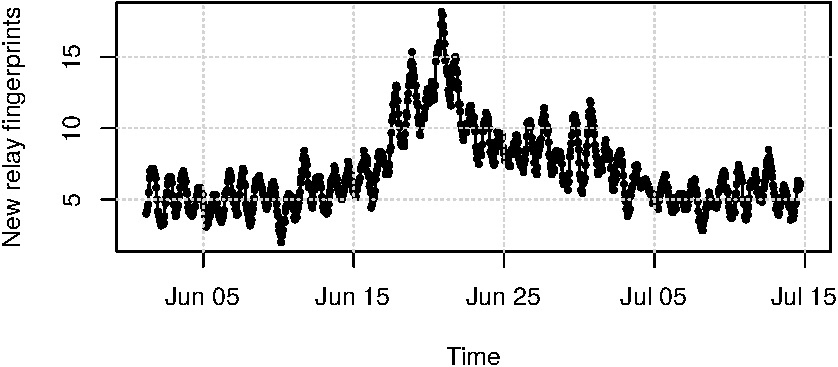
\includegraphics[width=0.47\textwidth]{diagrams/flat-hill.pdf}
	\caption{Flat hill in 2009.  Smoothed using moving average with a window
	size of 12.}
	\label{fig:flat-hill}
\end{figure}

\begin{figure}[t]
	\centering
	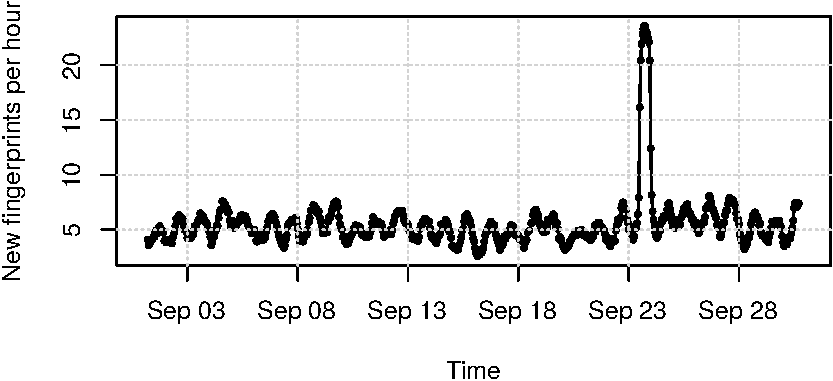
\includegraphics[width=0.47\textwidth]{diagrams/sudden-spike.pdf}
	\caption{Sudden spike in 2010.  Smoothed using moving average with a window
	size of 12.}
	\label{fig:sudden-spike}
\end{figure}

To quantify the churn rate $\sigma$ between two subsequent consensus documents,
we adapt the formula proposed by Godfrey et al.~\cite{Godfrey2006a}.  Godfrey et
al.'s formula yields a single churn value that captures both, new and gone
systems.  That means that an unusually low number of gone systems could ``hide''
an unusually high number of new systems---an undesired property for a system
that should highlight abnormal changes.  To address this issue, we split the
formula in two parts and create a time series for new relays ($\sigma_{n}$) as
well as for gone relays ($\sigma_{g}$).  $C_{t}$ is the network consensus at
time $t$, and $\setminus$ denotes the complement between two consensuses, i.e.,
the number of relays that is in one consensus, but not the other.

\begin{equation}
\sigma_{n} = \frac{\lvert C_{t} \setminus C_{t-1} \rvert}
{\textrm{max}\{\lvert C_{t-1} \rvert, \lvert C_{t} \rvert \}}
\end{equation}

\begin{equation}
\sigma_{g} = \frac{\lvert C_{t-1} \setminus C_{t} \rvert}
{\textrm{max}\{\lvert C_{t-1} \rvert, \lvert C_{t} \rvert \}}
\end{equation}

$\sigma_{n}$ and $\sigma_{g}$ are bounded to the interval $[0, 1]$.  A churn
value of 0 indicates no change between two subsequent consensuses whereas a
churn value of 1 indicates a complete network turnover.  Determining
$\sigma_{n,g}$ for the sequence $C_{t}, C_{t-1}$, $C_{t-2}$, \ldots, yields a
time series of churn values that can readily be inspected for abnormal spikes as
the one in Figure~\ref{fig:sudden-spike}.  To detect changes in the underlying
trend, we can smooth $\sigma_{n,g}$ using a simple moving average $\lambda$,

\begin{equation}
\lambda = \frac{1}{w} \cdot \sum_{i=0}^{w} \sigma_{i}
\end{equation}

As we increase the window size $w$, we are able to detect more subtle changes in
the underlying trend.  In an operating setting, we believe that this parameter
should be kept secret because otherwise it would help attackers to stay under
the radar.  Refer to Section~\ref{sec:secrecy} for a more comprehensive
discussion.  If $\lambda$ or $\sigma_{n,g}$ exceed a manually defined threshold,
an alert is raised.

\mynote{We could plot the number of alerts we would get for a sequence of
thresholds.}

\subsection{Uptime matrix}
\label{sec:uptime-matrix}
An unexpectedly high churn rate can indicate a significant network event, but it
does not reveal \emph{which relays} are responsible for this event.  It captures
the state of the network, but not of individual relays.  To bridge this gap, we
now propose an analysis technique for the uptime of single relays.

We now take a step back to understand why relay uptimes are relevant.  For
convenience, attackers are likely to administer their Sybil relays in parallel,
i.e., update, configure, and reboot them simultaneously.  This is reflected in
the hourly uptime of Tor relays.  If an attacker decides to install an operating
system upgrade on all of her Sybils, we might observe a cluster of relays going
offline and back online all at the same time.  To isolate such events, we are
comparing \emph{uptime patterns} of Tor relays.  Relays featuring a similar
uptime pattern are more likely to be under common control than relays with a
distinct uptime pattern.

We represent uptime patterns as a binary sequences.  Every hour, when a new
consensus is published, we append a new data point to the sequence for each Tor
relay.  It is tempting to then use the Hamming distance to quantify the
similarity between two relays.  The Hamming distance is the amount of positions
at which two strings of equal length differ.  This, however, does not perfectly
capture our intuition as we show in Figure~\ref{fig:uptime-pattern}.  Relay $B$
and $C$ have the same Hamming distance to relay $A$: two.  Intuitively, however,
we consider relay $B$ to be more similar to relay $A$ than is $C$ because it
does not exhibit the uptime sequence at hour seven and eight.  We account for
this by increasing a \emph{deviation amplifier} as two uptime sequences
continue to diverge (see Algorithm~\ref{alg:uptime}).  As long as two sequences
keep deviating, our deviation amplifier is increased by 0.1 until it reaches 1.
As soon as two sequences converge again, the deviation error is reset to 0.
Finally, we divide the distance by the sequence length to normalize it to the
interval $[0, 1]$.  According to this algorithm, relay $A$ and $B$ in
Figure~\ref{fig:uptime-pattern} have a similarity of 0.1 + 0.1 while $A$ and $C$
have a similarity of 0.1 + 0.2.

\mynote{Uptime sequences in Algorithm~\ref{alg:uptime} should probably deviate
exponentially rather than linearly.}

\begin{figure}[t]
\centering
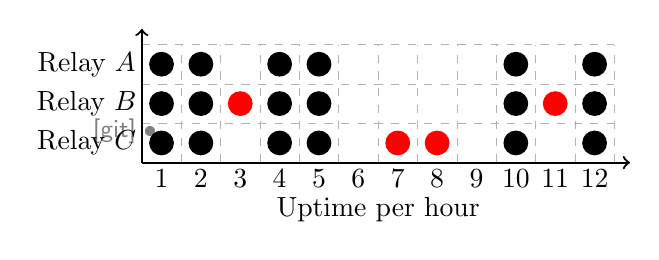
\begin{tikzpicture}
\draw[help lines, color=gray!60, dashed, step=0.5] (0,0) grid (6,1.5);
\draw[->,thick] (0,0)--(6.2,0);
\draw[->,thick] (0,0)--(0,1.7);

% Y labels.
\node at (-0.7,1.25) {Relay $A$};
\node at (-0.7,0.75) {Relay $B$};
\node at (-0.7,0.25) {Relay $C$};

% X labels.
\node at (0.25, -0.2) {1};
\node at (0.75, -0.2) {2};
\node at (1.25, -0.2) {3};
\node at (1.75, -0.2) {4};
\node at (2.25, -0.2) {5};
\node at (2.75, -0.2) {6};
\node at (3.25, -0.2) {7};
\node at (3.75, -0.2) {8};
\node at (4.25, -0.2) {9};
\node at (4.75, -0.2) {10};
\node at (5.25, -0.2) {11};
\node at (5.75, -0.2) {12};

\node at (3, -0.6) {Uptime per hour};

% Relay A.
\filldraw[black] (0.25,1.25) circle (0.15);
\filldraw[black] (0.75,1.25) circle (0.15);

\filldraw[black] (1.75,1.25) circle (0.15);
\filldraw[black] (2.25,1.25) circle (0.15);

\filldraw[black] (4.75,1.25) circle (0.15);

\filldraw[black] (5.75,1.25) circle (0.15);

% Relay B.
\filldraw[black] (0.25,0.75) circle (0.15);
\filldraw[black] (0.75,0.75) circle (0.15);
\filldraw[red]   (1.25,0.75) circle (0.15);
\filldraw[black] (1.75,0.75) circle (0.15);
\filldraw[black] (2.25,0.75) circle (0.15);

\filldraw[black] (4.75,0.75) circle (0.15);
\filldraw[red]   (5.25,0.75) circle (0.15);
\filldraw[black] (5.75,0.75) circle (0.15);

% Relay C.
\filldraw[black] (0.25,0.25) circle (0.15);
\filldraw[black] (0.75,0.25) circle (0.15);

\filldraw[black] (1.75,0.25) circle (0.15);
\filldraw[black] (2.25,0.25) circle (0.15);

\filldraw[red]   (3.25,0.25) circle (0.15);
\filldraw[red]   (3.75,0.25) circle (0.15);

\filldraw[black] (4.75,0.25) circle (0.15);

\filldraw[black] (5.75,0.25) circle (0.15);
\end{tikzpicture}

\caption{Uptime pattern of three relays.  Intuitively, relay $B$ is more
similar to relay $A$ than is relay $C$, but the Hamming distance is two for
both patterns.}
\label{fig:uptime-pattern}
\end{figure}

\begin{algorithm}[t]
\SetKwData{Dist}{dist}
\SetKwData{Amp}{amp}
\SetKwData{Hours}{hours}
\SetKwData{Result}{result}
\SetKwInOut{Input}{input}
\SetKwInOut{Output}{output}

\Input{$A$ and $B$, two uptime patterns}
\Output{$\Result$}
\BlankLine
$\Dist \leftarrow 0$\;
$\Amp \leftarrow 0$\;
\ForEach{$t \in \Hours$}{
    \eIf{$A_{t} \ne B_{t}$}{
        \If{$\Amp < 1$}{
            $\Amp \leftarrow \Amp + 0.1$\;
        }
    $\Dist \leftarrow \Dist + \Amp$\;
    }{
        $\Amp \leftarrow 0$\;
    }
}
$\Result \leftarrow \Dist / \lvert \Hours \rvert$\;
\caption{Our algorithm to quantify the similarity between the uptime pattern
of two relays $A$ and $B$.}
\label{alg:uptime}
\end{algorithm}

We employ Algorithm~\ref{alg:uptime} in a visualization that sybilhunter can
generate for a given set of consensuses.  The visualization is a bitmap whose
rows denote hours, and whose columns denote relays.  Every pixel in the image
represents the uptime status of a given relay.  If the pixel is black, the relay
is online, and if it is white, it is offline.  Note that this type of
visualization was first proposed by Fifield on the Tor bug
tracker~\cite{Fifield2014a}.  Similar to Fifield, we sort columns to group
similar uptime patterns together.  Our first sorting criteria is the amount of
hours a relay was online, and our second criteria is the median value of the
online sequence.  Figure~\ref{fig:uptime-matrix} gives an example, illustrating
the uptime patterns for relays in September 2011.  As columns increase, so does
the uptime of relays, until they are almost always online.  Sybils with similar
uptimes manifest as solid ``blacks'' in this type of visualization.  Refer to
Section~\ref{sec:fingerprint-anomalies} for examples.

\begin{figure}[t]
	\centering
	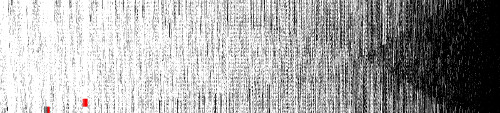
\includegraphics[width=0.48\textwidth]{diagrams/2011-09-uptimes-truncated.jpg}
	\caption{The uptime matrix for a subset of all Tor relays in September 2011.
		Every row in the image represents one consensus, and every column
		represents one relay.  As a result, every pixel denotes the uptime
		status of a given relay at a given hour.  Black pixels mean ``online,''
		white pixels mean ``offline.''  Green rows denote missing consensuses
		and red blocks denote possible Sybil groups.}
	\label{fig:uptime-matrix}
\end{figure}

Once the columns are sorted, we run our algorithm to determine the distance
between two subsequent uptime sequences.  If the distance is under our
threshold, we mark both uptime sequences as red, to make them easy to find in
manual analysis.

\subsection{Fingerprint analysis}
\label{sec:fingerprint-analysis}
The information a Tor client needs to connect to a hidden service is saved in
a distributed hash table (DHT) that consists of a subset of all Tor relays, the
hidden service directories (HSDirs).  A daily-changing set of six HSDirs are
responsible for a given hidden service.  Tor clients ask these HSDirs for
information about the hidden service they want to connect to.

A HSDir becomes responsible for a hidden service when its fingerprint
is closest to the descriptor ID that is derived from the hidden service's public
key, a time stamp, and additional information.
% https://gitweb.torproject.org/torspec.git/tree/rend-spec.txt:231
% descriptor-id = H(permanent-id | H(time-period | descriptor-cookie | replica))
Note that the DHT and all its HSDirs is known and it is also possible to
calculate which index in the fingerprint ring will be used by a hidden service
at a future point in time~\cite{Biryukov2013a}.  Attackers can exploit this
knowledge by generating identity keys until their fingerprint is close to the
hidden service's index, thus becoming responsible for it.  To save resources,
an attacker can run a single, physical Tor relay and generate a new identity
periodically.

We detect relays that change their fingerprint frequently by maintaining a
lookup table that maps a relay's IP addresses to a list of all fingerprints we
have seen it use.  We order the lookup table by the relays that changed the
fingerprints the most, and output the results.

\mynote{Elaborate.}

\subsection{Nearest-neighbor search}
\label{sec:nearest-neighbor}
We frequently found ourselves in a situation where exitmap discovered a
malicious exit relay and we were trying to find similar, potentially associated
relays.  This involved extensive manual work, which we soon started to automate.
In particular, we needed an algorithm for nearest-neighbor search: given a
``seed'' relay, what are its $n$ nearest neighbors?

A naive implementation would compare the seed relay to all other relays in the
consensus, which scales linearly.  We can do better by using metric trees, which
guarantee $\mathcal{O}(\textrm{log} n)$ lookup.  Metric trees are a type of data
structure to index data in metric spaces.  Metric trees require a distance
metric in the mathematical sense, i.e., a number of conditions to be met (see
Appendix~\ref{sec:metric}), which are not always satisfied by ad-hoc metrics.
% In particular, the triangle inequality\footnote{The triangle inequality, $d(x,
% z) \le d(x, y) + d(y, z)$, states that the distance between two points is at
% least equal to a ``detour'' over a third point.} can be difficult to meet when
% working in non-Euclidean space.

\mynote{Explain more rigorously.}

We use the Levenshtein distance as distance metric.  It operates on strings and
determines the minimum amount of modifications---insert, delete, and
modify---that are necessary to turn string $s_{1}$ into $s_{2}$.  The
Levenshtein distance can handle strings of different length, and satisfies the
triangle inequality, i.e., we are free to use it in a metric tree.

As concrete metric tree implementation, we use the vantage point tree
(vp-tree)~\cite{Yianilos1993a}.  It recursively divides the given data into two
partitions; one that is close to the seed point according to a threshold,
and one that is not.  The vp-tree must first be built for the given data, and it
is then ready to perform nearest neighbor searches.

\mynote{Talk about how long it takes to build the tree.}

In our implementation, building a vp-tree for 6,235 relays takes approximately
10 seconds.\footnote{Again, measured on a single Intel Core i7 2.9 GHz CPU.}
Subsequent nearest-neighbor lookups finish almost instantly.

\mynote{Still need to compare this to naive $n^{2}$ search.}

\subsection{Blocking Sybils}
Once we isolated a Sybil group, and concluded that it appears to be harmful, we
reported it to The Tor Project.  There are currently two ways for directory
authorities to block relays, controlled by the options \texttt{AuthDirReject}
and \texttt{AuthDirInvalid}.  The former removes a relay from the consensus.
The latter takes away a relay's \texttt{Valid} flag.  While the relay is still
listed in the consensus, clients will not consider it for path selection.

The majority of directory authorities, i.e., four out of eight, must agree on
either \texttt{AuthDirReject} or \texttt{AuthDirInvalid} be set for a relay.
Only then will the block become active.  This mechanism is meant to distribute
the power of removing relays into the hands of a diverse set of people.  We
elaborate on our experience with this process in Section~\ref{sec:operational}.

\subsection{Meaningful results}
Systems that employ complex and opaque analysis techniques to expose security
incidents frequently suffer from what Sommer and Paxson call the \emph{semantic
gap}~\cite[\S III.C]{Sommer2010a}, i.e., a system's output is difficult to act
upon as its meaning is unclear.  Our tools automate the detection of Sybils,
but the process of blocking them involves human interaction, which is why we
took special care to consider the semantic gap.

We avoid the use of opaque classification methods as their output (often a
distance in high-dimensional vector space) is difficult to interpret.  Instead,
we rely on straightforward metrics such as the Levenshtein distance.
Figure~\ref{fig:visualization} further illustrates a visualization that we
developed for exploratory analysis, which is meant to complement automated
analysis.  The graph shows the similarities (edges) between four Tor relays
(vertices).

\begin{figure}[t]
	\centering
	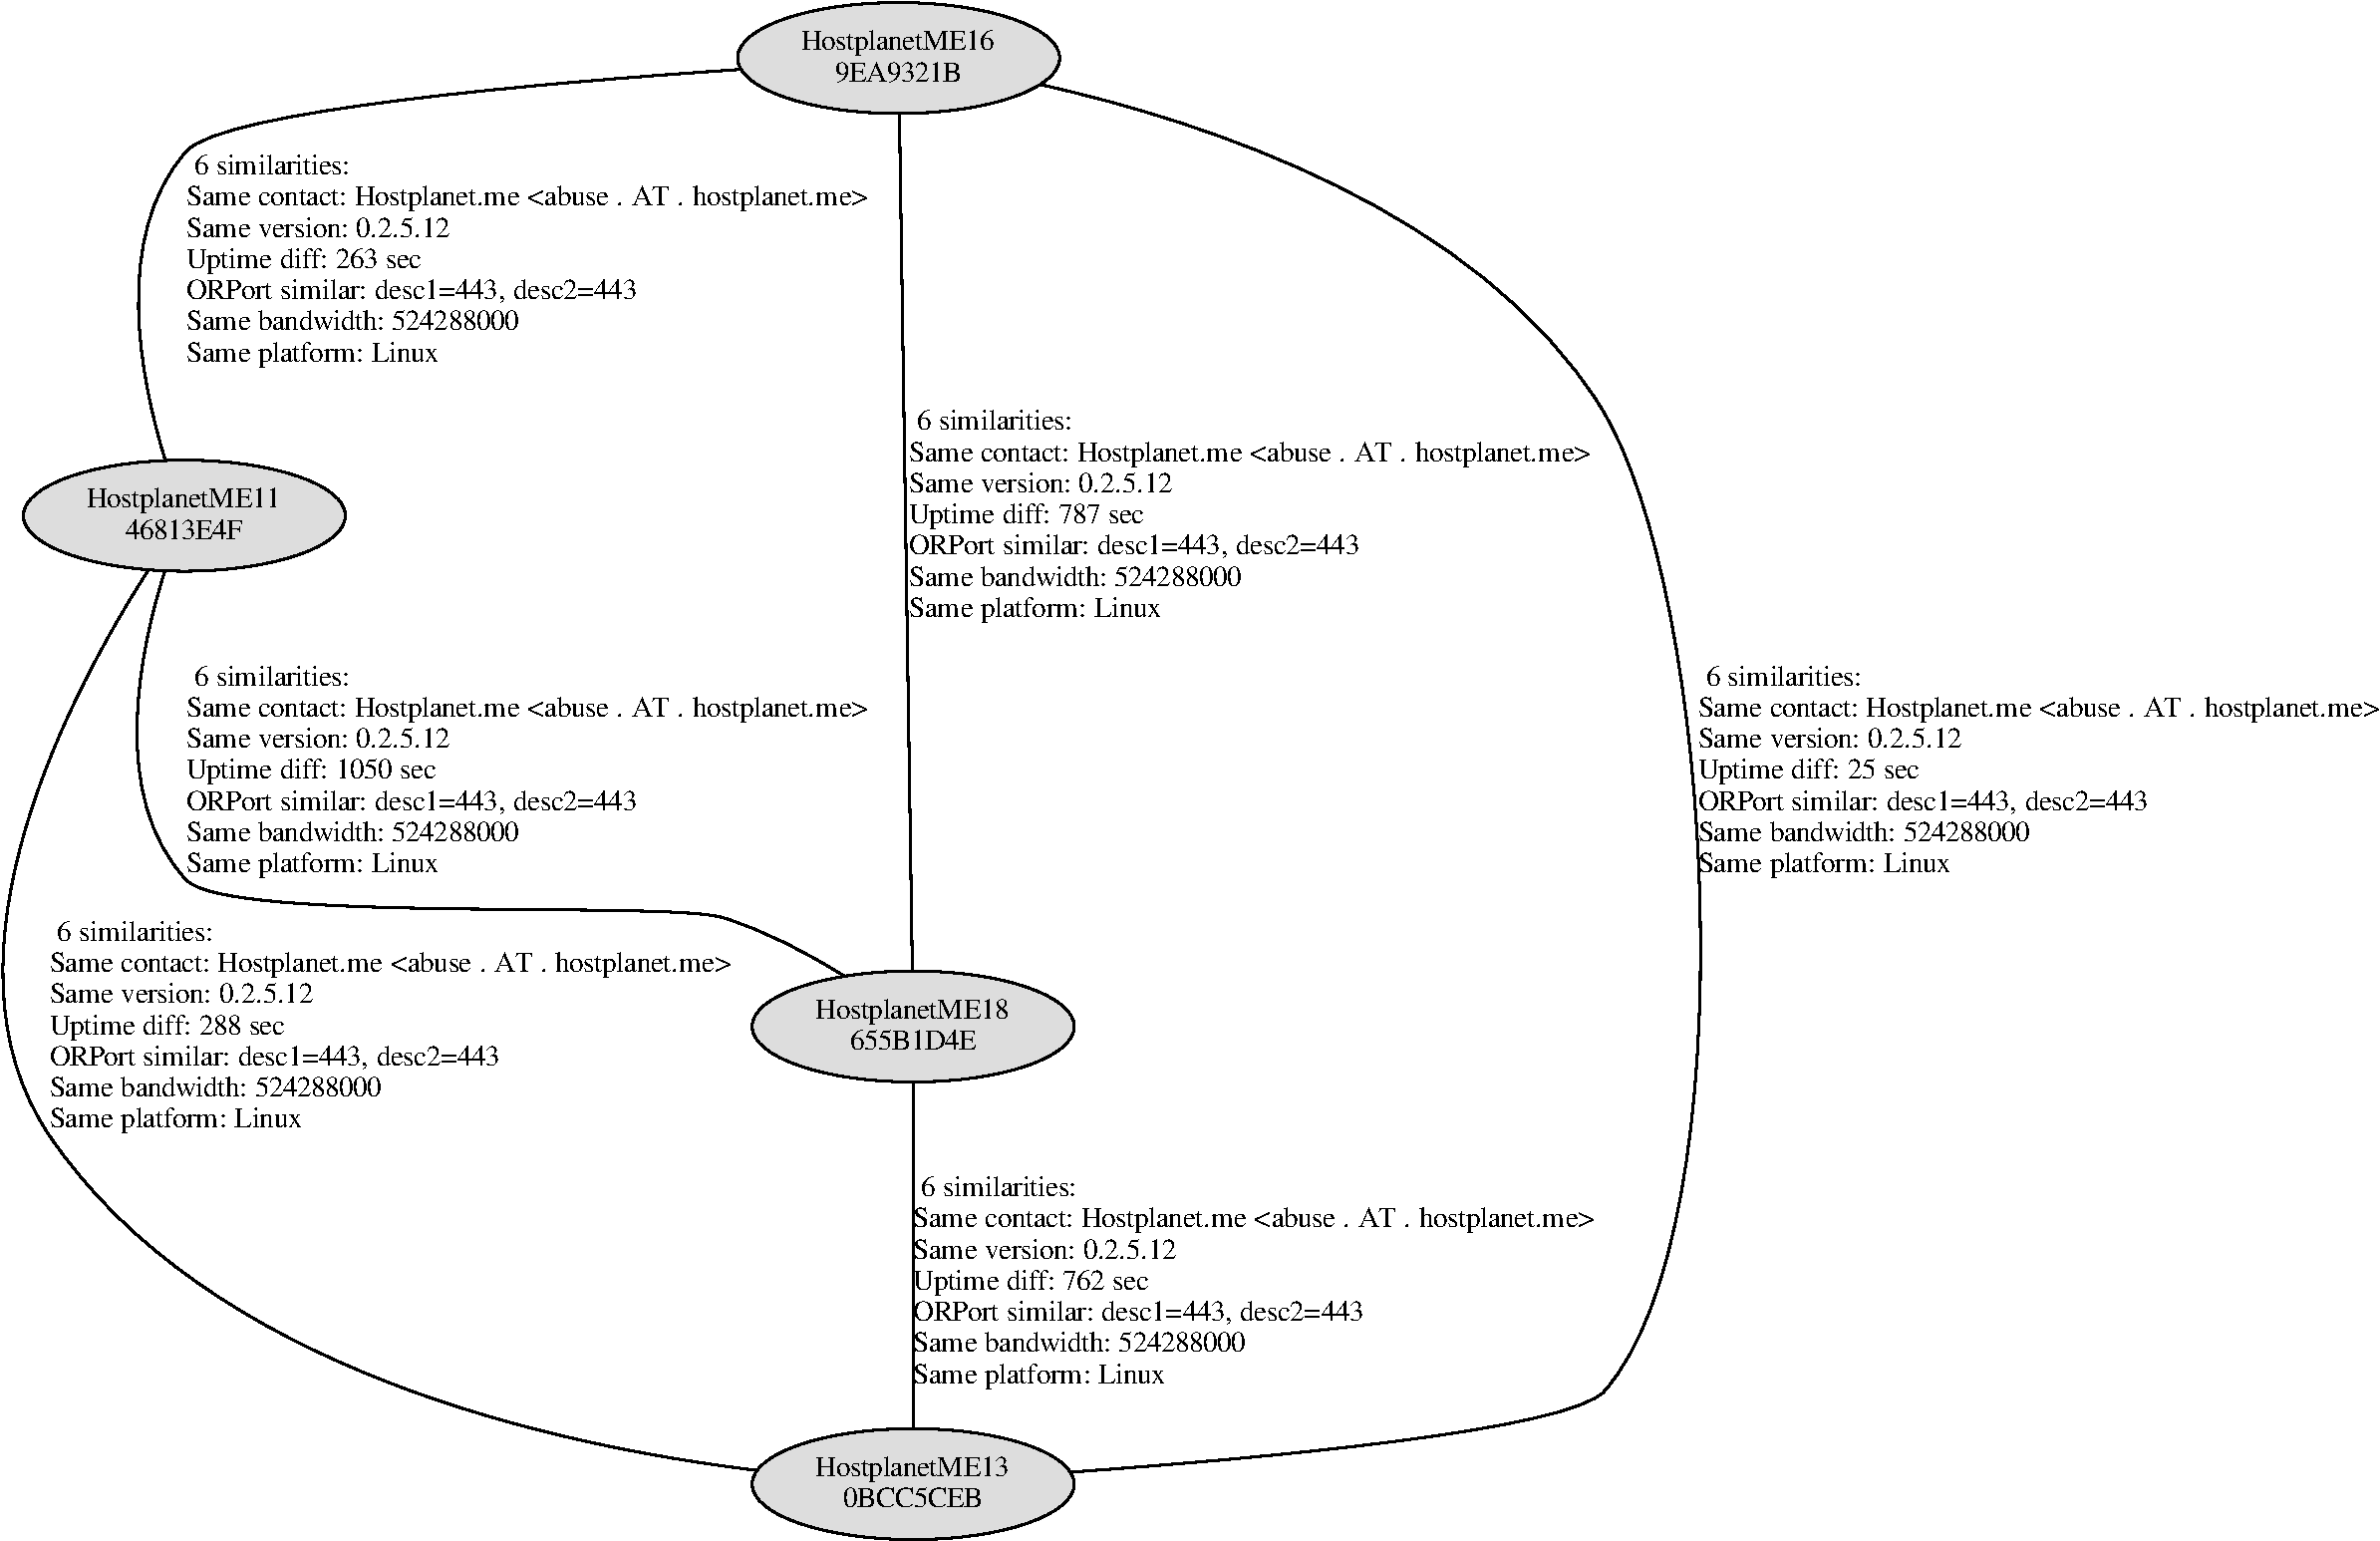
\includegraphics[width=0.42\textwidth]{diagrams/visualization.pdf}
    \caption{Visualization of a Sybil cluster.  Vertices represent Tor relays
    and edges show the similarities between them.}
	\label{fig:visualization}
\end{figure}


\section{Evaluation and results}
\label{sec:results}
We now discuss the results we obtained by applying the techniques we presented
above on the datasets we presented in Section~\ref{sec:datasets}.  We begin by
presenting the results of the churn rate analysis (\S~\ref{sec:churn}), followed
by the uptime analysis (\S~\ref{sec:uptime}), and the fingerprint analysis
(\S~\ref{sec:fingerprint-anomalies}).  Next, we characterize the most
interesting Sybils we found in our analysis (\S~\ref{sec:sybil_groups}).
Finally, we evaluate our nearest-neighbor search (\S~\ref{sec:accuracy}) and the
computational performance of all our analysis techniques
(\S~\ref{sec:performance}).

\subsection{Churn rate analysis}
\label{sec:churn}
We determined the churn rates of two subsequent consensuses for all 69,133
consensuses.  There are 158 gaps in the archived data, so we ended up with
$68,975 \cdot 2 = 137,950$ churn values for both time series.
Figure~\ref{fig:churn-density} illustrates a density plot that shows the
distribution of all these churn values, 99.97\% of which are in the interval
$[0, 0.1]$.  The diagram further features 37 vertical dotted lines that mark
outliers above 0.1.  Table~\ref{tab:churn-dist} gives an overview of our time
series statistics.

\begin{figure}[t]
	\centering
	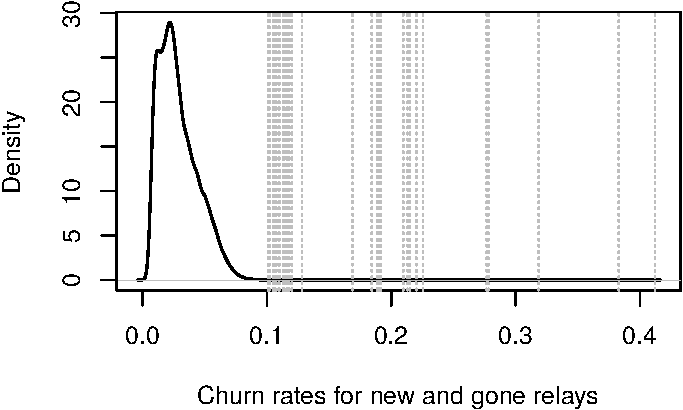
\includegraphics[width=\linewidth]{diagrams/churn-density.pdf}
	\caption{Density of all churn values for new and gone relays.  For both
	time series, 37 churn rates over eight years exceeded 0.1.  The dotted
	vertical lines mark all outliers.}
	\label{fig:churn-density}
\end{figure}

\begin{table}[t]
	\centering
	\begin{tabular}{ccccccc}
	\textbf{Churn type} & \textbf{Min.} & \textbf{Median} & \textbf{Mean} & \textbf{Max.} \\
	\hline
	New & 0.000 & 0.026 & 0.029 & 0.319 \\
	Gone & 0.003 & 0.025 & 0.029 & 0.412 \\
	\end{tabular}
	\caption{Summary of the distribution of churn rates for all consensuses
	since 2007.}
	\label{tab:churn-dist}
\end{table}

Figure~\ref{fig:2008-08} illustrates the churn rates for August 2008, featuring
our biggest anomaly.  On August 19, 822 relays left the network, resulting in a
sudden spike of the churn rate, and a trend increase in the time series.  The
spike was caused by the switch from consensus method three to four, which
happened on August 19, 2008.  The changelog says that in consensus method four,
routers that don't have the \texttt{Running} flag are no longer listed in the
consensus.

\begin{figure}[t]
	\centering
	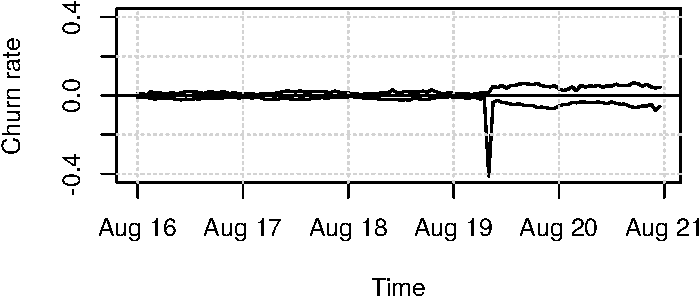
\includegraphics[width=\linewidth]{diagrams/2008-08.pdf}
	\caption{On August 19, 822 relays suddenly left the Tor network, resulting
	in a churn rate spike, and a time series increase.  The event was caused by
	the switch from consensus method three to four.}
	\label{fig:2008-08}
\end{figure}

\mynote{Still need to discuss other outliers.}

\subsection{Uptime analysis}
\label{sec:uptime}
We generated relay uptime illustrations for every month since 2007, resulting in
93 uptime visualizations.\footnote{All images are available online, on the following
onion service: \url{http://qviewr5ittnqdcvi.onion}.}
We now discuss a subset of these images that
contain particularly interesting patterns.

Figure~\ref{fig:2010-06-planetlab} shows June 2010, featuring a clear ``Sybil
block'' on the left side.  The Sybils belonged to a researcher who, as
documented by The Tor Project~\cite{progressreport}, started 512 Tor relays on
PlanetLab for research on scalability.  Our manual analysis could verify this.
The relays were easy to identify because their nicknames suggested that they
were hosted on PlanetLab, containing strings such as ``planetlab,'' ``planet,''
and ``plab.''  Note the small height of the Sybil block, indicating that the
relays were not online for a long time.

\begin{figure}[t]
	\centering
	
\includegraphics[width=\linewidth]{diagrams/planetlab-uptimes.jpg}
	\caption{In June 2010, a researcher started 512 Tor relays on PlanetLab for,
		as The Tor Project documented, ``their research into cloud computing and
		scaling effects''~\cite{progressreport}.  As illustrated by the easily
		visible red bar on the left, the relays were only online for a short
		while.}
	\label{fig:2010-06-planetlab}
\end{figure}

Figure~\ref{fig:2012-08-steppattern} features a curious ``step pattern'' for
approximately 100 relays, all of which were located in Russia and Germany.  The
relays appeared in December 2011, and started exhibiting the diurnal step
pattern (nine hours uptime followed by 15 hours downtime) in March 2012.  All
relays had similar nicknames, consisting of eight seemingly randomly-generated
characters.  In April 2013, the relays finally disappeared.

\begin{figure}[t]
	\centering
	
\includegraphics[width=\linewidth]{diagrams/2012-08.jpg}
	\caption{August 2012 featured a curious ``step pattern,'' caused by
	approximately 100 Sybils.  Out of 24 hours, the relays were online for only
	nine hours.}
	\label{fig:2012-08-steppattern}
\end{figure}

Figure~\ref{fig:2014-04-heartbleed} shows the effect of the Heartbleed
incident~\cite{Durumeric2014a} on the Tor network.  Several days after the
incident, The Tor Project decided to block all relays that haven't generated new
key pairs.  The large red block in the middle of the picture illustrates when
the biggest part of the block became active, rejecting approximately 1,700 Tor
relay fingerprints.
% $ wc -l dirauth-conf/approved-routers.d/bleeding-edges.conf
% 1779 dirauth-conf/approved-routers.d/bleeding-edges.conf

\begin{figure}[t]
	\centering
	
\includegraphics[width=\linewidth]{diagrams/heartbleed-uptimes.jpg}
	\caption{April 2014, the month the Heartbleed bug was discovered.
		The large block in the middle of the diagram happened because The
		Tor Project eventually rejected a large number of relays that did not
		change their keypairs in time.}
		\label{fig:2014-04-heartbleed}
\end{figure}

Figure~\ref{fig:2014-12-lizard} illustrates the largest Sybil group to date,
comprising 3,347 Tor relays that an attacker started in the Google cloud in
December 2014.  Because of its magnitude, the attack was spotted almost
instantly, and The Tor Project was quick to remove the offending relays nine
hours after the appeared.

\begin{figure}[t]
	\centering
	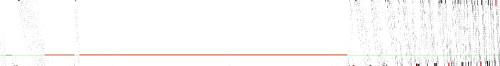
\includegraphics[width=\linewidth]{diagrams/lizard-uptimes.jpg}
	\caption{December 2014, when a group of people started several hundred Tor
	relays in the Google cloud.  The relays were only online for a small number
	of hours because they were promptly rejected by The Tor Project.}
	\label{fig:2014-12-lizard}
\end{figure}

\subsection{Fingerprint anomalies}
\label{sec:fingerprint-anomalies}
We determined how often all Tor relays changed their fingerprint from 2007 to
2015.  Figure~\ref{fig:fingerprints} illustrates the amount of fingerprints
(y-axis) we have observed for the 1,000 Tor relays (x-axis) that changed their
fingerprint the most.  All these relays changed their fingerprint at least ten
times.  Twenty one relays changed their fingerprint more than 100 times, and the
relay at the very right end of the distribution changed its fingerprint 936
times.  This relay's nickname was ``openwrt,'' suggesting that it was a home
router that was rebooted regularly.  It was running from August 2010 to December
2010.

\begin{figure}[t]
	\centering
	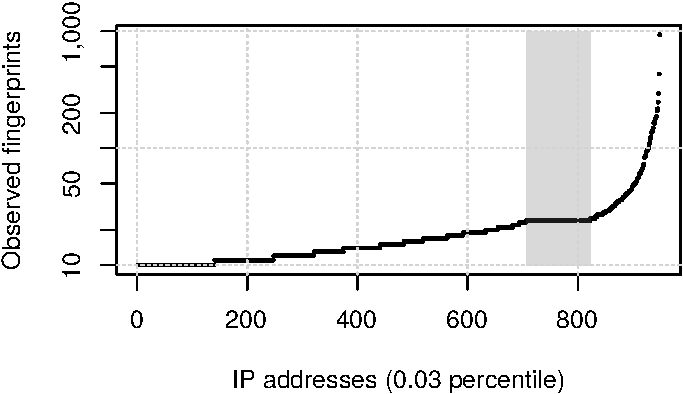
\includegraphics[width=\linewidth]{diagrams/fingerprints.pdf}
	\caption{The amount of observed fingerprints for the 1,000 relays that
	changed their fingerprints the most.  Note the curious plateau in the shaded
	area between index 707 and 803---a Sybil group that changed their
	fingerprint exactly 24 times.}
	\label{fig:fingerprints}
\end{figure}

Figure~\ref{fig:fingerprints} further contains a peculiar plateau, shown in the
shaded area between index 707 and 803.  This plateau was caused by a group of
Sybils, hosted in Amazon EC2, that changed their fingerprint exactly 24 times.

We also found that many IP addresses in the range 199.254.238.0/24 changed their
fingerprint frequently.  We contacted the owner of the address block and were
told that the block used to host VPN services.  Apparently, several people
started Tor relays and since the VPN service would not assign permanent IP
addresses, the Tor relays would periodically change their address, causing the
churn we observe.

\subsection{Sybil characterization}
\label{sec:sybil_groups}
Table~\ref{tab:sybils} contains all the Sybil groups we identified.  For every
group, we document when it first appeared in the Tor network, its ``name,''
size, and a description of its characteristics.  In addition, we now discuss the
most interesting Sybil groups in greater detail.

\begin{table*}[t]
\centering
\begin{tabular}{l c c p{10cm}}
\textbf{First seen} & \textbf{Group ID} & \textbf{\# of relays} & \textbf{Characteristics} \\
\hline
\ldots & \ldots & 6 & Disable STARTTLS for SMTP. \\
2015-07-10 & DenkoNet & 58 & Hosted on Amazon AWS.  Only online for one consensus. \\
2015-07-02 & cloudvps & 55 & \ldots \\
2015-06-29 & onion rewrite & 55 & Transparent onion URL rewriting. \\
2015-06-17 & 1jabberat & \ldots & \ldots \\
2015-06-05 & hsdirscanner2 & 105 & Scanning HSDirs. \\
2015-06-03 & abcd & 28 & Changing fingerprints. \\
2015-05-29 & facebook hsdirs & 6 & Became HSDirs responsible for facebook.  \\
2015-05-20 & hsdirscanner1 & 102 & Scanning HSDirs. \\
2015-04-22 & sigaint & 83 & Targeting (at least) sigaint.org. \\
2015-03-11 & bitcoin-redirect & 24 & Attacking Bitcoin sites by redirecting to own web server. \\
\ldots & default & many & Likely a Windows-powered botnet.  The group
features wide, geographical distribution, which is uncommon for typical Tor
relays. \\
% Shared: nickname, IP address, port, platform, version.
2014-12-30 & Anonpoke & 284 & \ldots\\
2014-12-26 & FuslVZTOR & 246 & The relays showed up only hours after the
LizardNSA incident. \\
2014-12-26 & LizardNSA & 3,347 & A hacker group publicly claimed to be
responsible for the attack.  All relays were hosted in the Google cloud and The
Tor Project removed them within hours. \\
2013-02-03 & AmazonEC2 & \ldots & Changed their fingerprint exactly 24 times. \\
2014-01-04 & fdcserver & \ldots & \ldots \\
2010-10-05 & trotsky & \ldots & \ldots \\
2010-06-26 & planetlab & 512 & According to a report from The Tor
Project~\cite{progressreport}, a researcher started these relays to learn more
about scalability effects.  The relays were online for approximately two days. \\
2008-09-26 & torism & 10 & \ldots \\
\end{tabular}
\caption{Sybil groups identified by our system.  Our raw data is available
online. \emph{URL redacted for anonymization.}}
\label{tab:sybils}
\end{table*}

\subsubsection{default}
This Sybil group, named after the shared nickname ``default,'' has been around
since 2011 (see Figure~\ref{fig:default-over-time}) and consists of
Windows-powered relays only.  All members run Tor in version 0.2.4.X, many
releases are older than Sep. 2014.  We extracted relays by filtering consensuses
for nicknames that are set to ``default,'' onion routing ports set to 443, and
directory ports set to 9030.  The group features high IP address churn.  For
Oct. 2015, we found ``default'' relays in 73 countries, with the top three
countries being Germany~(50\%), Russia~(8\%), and Austria~(7\%).  The majority
of these relays, however, has little uptime.
Figure~\ref{fig:default-sybils-uptime} shows the uptime matrix for ``default''
relays in Oct. 2015.  Many relays exhibit a diurnal pattern, suggesting
that they are powered off regularly---as it often is the case for desktop PCs.

\begin{figure}[t]
	\centering
	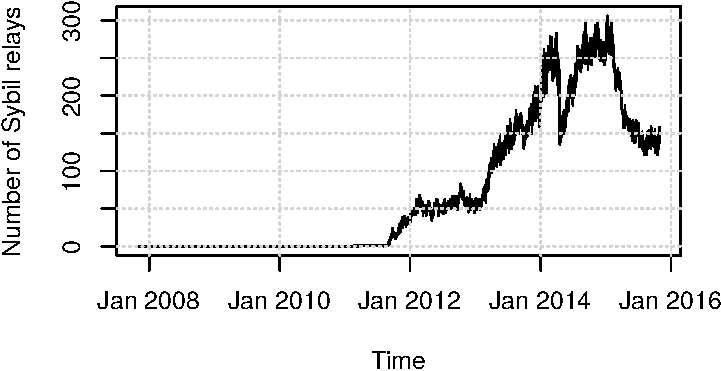
\includegraphics[width=0.47\textwidth]{diagrams/default-over-time}
	\caption{The amount of relays that we deem part of the Sybil group
	``default'' over time.  The relays surfaced in Sep. 2011.}
	\label{fig:default-over-time}
\end{figure}

To get a better understanding of the amount of ``default'' relays over time, we
analyzed all consensuses, extracting the number of relays whose nickname was
``default,'' whose onion routing port was 443, and whose directory port was
9001.  We did this for the first consensus every day and plot the result in
Figure~\ref{fig:default-over-time}.

The above suggests that some of these relays are running without the owner's
knowledge.  The relays don't fit the pattern of Sefnit (a.k.a.
Mevade)~\cite{sefnit} and Skynet~\cite{skynet}, two pieces of malware that use
an onion service as command and control server.  Nevertheless, we believe that
these could could be part of a botnet.

\subsubsection{LizardNSA}
All relays were hosted in the Google Cloud, and only online for nine hours,
until the directory authorities started rejecting them.  The majority of
machines were middle relays (96\%), but the attackers also started some exit
relays (4\%).  The Sybils were set up to be onion service directories, but the
relays were taken offline before they were assigned the \texttt{HSDir} flag.  If
all relays would have obtained the \texttt{HSDir} flag in time, they would have
constituted almost 50\% of all onion service directories; the median number of
onion service directories on Dec. 26 was 3,551.

\subsubsection{FuslVZTOR}
All machines were middle relays and hosted in 212.38.181.0/24, a VPS provider's
network in the UK.  The directory authorities started rejecting the relays five
hours after they were first seen.  The relays advertized the default bandwidth
of 1 GiB/s and used seemingly randomly determined ports.  Other than happening
in parallel to the LizardNSA attack, there is no reason to believe that both
incidents are related.

\subsubsection{Anonpoke}
The relays were online for four hours until they were rejected.  All relays were
hosted by a VPS provider in the US, with the curious exception of a single relay
that was hosted in the UK, and running a different Tor version.  The relays
advertized the default bandwidth of 1 GiB/s on port 9001 and 9030.  All relays
were middle relays and running as directory mirror.  All Sybils were configured
to be an onion service directory, but did not manage to get the flag in time.

\subsubsection{PlanetLab}
A set of relays that used a variation of the strings ``planet'', ``plab'',
``pl'', and ``planetlab'' as their nickname.  The relays' exit policy allowed
ports 6660--6667, but they did not get the \texttt{Exit} flag.  The Sybils were
online for three days and then removed by The Tor Project, as mentioned in a
blog post~\cite{planetlab}.  The blog post further says that the relays were run
by a researchers.

% \subsubsection{Bitcoin}
% The ones that are stealing bitcoins.
% 
% Look at blockchain and figure out how much they stole.

\subsection{Accuracy of nearest-neighbor search}
\label{sec:accuracy}
A proper evaluation of our algorithm's classification performance requires
ground truth, i.e., Sybil relays that are \emph{known} to belong together.  All
we have, however, are Sybils that we \emph{believe} belong together.  We can use
this dataset as ground truth, but the resulting performance scores are likely an
overestimate of our algorithm's true performance because we manually tuned it to
consider the features that we believe our powerful Sybil predictors.

% We can (ab)use MyFamily data as ground truth.
In addition to our Sybil dataset, relay families can serve as ground truth.  A
relay family is a set of Tor relays that is controlled by one operator, and is
configured to express this mutual relationship in the family members'
configuration file.  In a way, relay families can be seen as benign Sybils.  Tor
clients never use more than one member of a family in their path to prevent
correlation attacks.  As of Nov.  2015, there are approximately \mynote{XXX}
families in the network, ranging from only two relays to \mynote{XXX} relays.
We can evaluate our algorithm by making it find the nearest neighbours of a
family member, which, ideally, should be its family members.  Again, using
families as ground truth is very likely to overestimate results because family
operators frequently configure their relays almost identically.  At the time of
this writing, a popular relay family uses the nicknames ``AccessNow000'' to
``AccessNow009,'' uses adjacent IP addresses, and identical contact information.
We expect the operators of malicious Sybils, however, to go out of their way to
obscure the relationship between their relays.

% Concrete MyFamily experiment.
To evaluate our nearest-neighbour search, we used all relay families that were
present in the first consensus that was published in Oct. 2015.  \mynote{Quick
overview of how many families were present.} For every relay that had a mutual
family relationship, we built a vantage point tree and then searched for its $n$
nearest neighbours where $n$ is the amount of mutual family relationships.
Basically, we evaluated how good our algorithm is at finding the relatives of a
family member.  We determined the precision and recall, both in the interval
$[0,1]$ and telling us how many of the nearest neighbours are family members
(precision) and how many family members were in the nearest neighbours (recall).
More formally, precision $\mathcal{P}$ is defined as
$$\mathcal{P} = \frac{|\textrm{\footnotesize Correctly identified Sybils}|}
{|\textrm{\footnotesize Uncorrectly identified Sybils}|}$$
and recall $\mathcal{R}$ is defined as
$$\mathcal{R} = \frac{|\textrm{\footnotesize Correctly identified Sybils}|}
{|\textrm{\footnotesize Correctly identified Sybils} \cap \textrm{\footnotesize Unidentified Sybils}|}.$$
For every family member in the consensus, we determined one precision and recall
value, respectively.  All values are illustrated in
Figure~\ref{fig:precision-recall}, showing precision on the x-axis and recall on
the y-axis.  The more points in the top right corner, the better is our
algorithm's classification performance.  Most value pairs were either $(1,1)$
(XXX\%) or $(0,0)$ (YYY\%).

\begin{figure}[t]
	\centering
	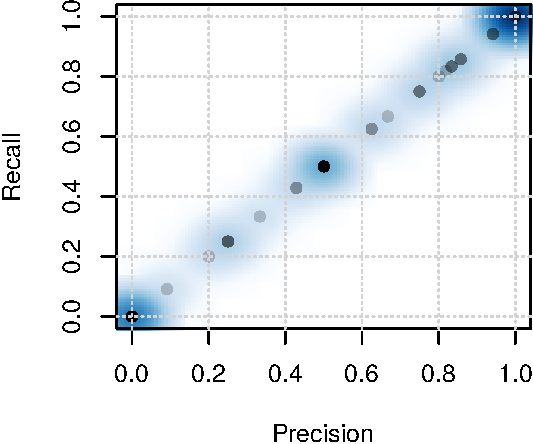
\includegraphics[width=0.32\textwidth]{diagrams/precision-recall.pdf}
	\caption{Precision and recall when our algorithm is applied on the relay
		family dataset.}
	\label{fig:precision-recall}
\end{figure}

We manually investigated some classification results and found that
\mynote{explain}.

\subsection{Computational cost}
\label{sec:performance}
We are interested in the computational cost of our analysis techniques.  Fast
methods lend themselves to being run hourly, for every new consensus, while
slower techniques must be run less frequent.  Table~\ref{tab:exp-deployment}
gives an overview of the runtime of our methods.\footnote{All performance
numbers were determined on an Intel Core i7-3520M CPU at 2.9 GHz.}  Note that we
placed our datasets on a solid state drive, to shift eliminate I/O as
performance bottleneck.

\begin{table}[t]
	\centering
	\begin{tabular}{lccc}
	\textbf{Method} & \textbf{Invocation} & \textbf{Analysis window} & \textbf{Run time} \\
	\hline
	Network churn & Hourly & One hour & $\sim$0.16s \\
	Nearest-neighbor & Daily & --- & $\sim$15s \\
	Fingerprint analysis & Daily & One month & $\sim$55s \\
	Uptime matrix & Daily & One month & $\sim$67s \\
	Similarity matrix & Daily & --- & XXX \\
	\end{tabular}
	\caption{The computational cost of our analysis techniques, measured in
	execution time.  Network churn analysis is very fast and can easily be run
	hourly while the creation of a similarity matrix takes more time and can be
	run daily.}
	\label{tab:exp-deployment}
\end{table}

The table columns contain, from left to right, our analysis technique, how often
we intend to run the technique, the technique's data time window, and how long
it takes to compute its output.  The calculation of network churn is very
fast---it takes as input only two consensus files---and can easily be done for
every network consensus.  Nearest-neighbour search takes approximately 15
seconds, most of which is spent building the vantage point tree.  We used
nearest-neighbour search for manual analysis, but it could be used
automatically.  Fingerprint and uptime analysis for one month work of consensus
files both take approximately one minute and can easily be run daily.
%Finally, computing a similarity matrix takes \mynote{XXX}.


\section{Discussion}
\label{sec:discussion}
Having presented and evaluated our techniques, we will now discuss the
transparency and secrecy tradeoff~(\S~\ref{sec:secrecy}), we reiterate our
work's limitations~(\S~\ref{sec:limitations}), and we discuss the role of cloud
providers in Sybil attacks~(\S~\ref{sec:cloud}).

\subsection{Balancing transparency and secrecy}
\label{sec:secrecy}
During the development of sybilhunter, we pondered what a reasonable balance
between transparency and secrecy should look like.  On the one hand, we want our
system design and code to be open, to stimulate scientific progress.  On the
other hand, a freely available implementation helps attackers evade our system
because they can first test and refine their attacks offline.

It seems difficult to achieve a setting analogous to Kerckhoffs' principle in
cryptography, stating that a system must be secure even if everything except the
key is known about it.  There is no key in our setting.  We can, however, divide
our system into the \emph{open} analysis framework and its \emph{secret}
parameters.  After all, the analysis framework is of primary interest to other
researchers, whereas its parameters are mere operational details.

Note that the authors of exitmap follow a similar philosophy by making available
exitmap's scanning framework~\cite{exitmap}, but sharing its modules only
privately.  This differentiation seems to be sustainable as attackers are
primarily interested in scanning modules, e.g., which URLs, protocols, and ports
are probed.

\subsection{Limitations}
\label{sec:limitations}
% We cannot detect all Sybils.  We can only make an effort.
We mentioned in Section~\ref{sec:threat_model} that we are unable to prevent all
Sybil attacks.  An adversary unconstrained by time and money will always be able
to add Sybils and eliminate redundancy in her Sybils' appearance and behavior.
This is known since Douceur showed in 2002 that the only way to prevent Sybil
attacks is a central authority that verifies network
participants~\cite{Douceur2002a}.  A central authority is unlikely to be viable
for the Tor network.  It would be in conflict with Tor's goal of distributing
trust and alienate relay operators.  As a result, detecting Sybils in the Tor
network is limited to making a best effort.

% We cannot determine the purpose of a Sybil cluster.
Finally, our approach is unable to determine the \emph{purpose} of a Sybil
attack.  In some cases, the purpose is obvious; for example, if a Sybil cluster
has the \texttt{Exit} flag and tampers with traffic, or if a cluster has the
\texttt{HSDir} flag and shares an unusually long fingerprint prefix.  In many
other cases, however, we rely on additional information to decide if a Sybil
cluster should be removed.  For example, Sybils originating from ``bulletproof''
ASes~\cite{Konte2015a}, showing signs of not running the tor reference
implementation, or spoofing information in their router descriptor could all
suggest malicious intent.  In the end, Sybil clusters have to be evaluated case
by case, and the benefits and disadvantages of blocking it have to be evaluated.

% We will now explore how costly a Sybil attack is in practice.  First, an
% adversary needs a number of systems to run Tor relays on.  These systems should
% be geographically distributed to maximize IP address diversity.  One option is
% to rent virtual private systems, starting at around \$3 per month for 1 Gbps.
% In 2011, the price for 1,000 compromised systems to install malware on (so
% called \emph{loads}) ranged from \$13 (in Asia) to \$125 (in the U.S.)\cite[\S
% 5]{Stone-Gross2011a}.

\subsection{Use and abuse of cloud providers}
\label{sec:cloud}
Some of the Sybil groups listed in Table~\ref{tab:sybils} were hosted in the
cloud.  Presumably, cloud-hosted relays are attractive to attackers because they
provide cheap, disposable, and hourly-billed platforms.  But does the bandwidth
contributed by cloud-hosted relays make up for the abuse?

To answer this question, we first calculated the amount of bandwidth contributed
by Tor relays that were located in the netblocks of three major cloud providers,
Amazon AWS~\cite{amazonaws}, Google Cloud Platform~\cite{googlecloud}, and
Microsoft Azure~\cite{azure}.  Note that the netblocks published by these cloud
providers can change over time, and are not archived.  As a result, we could
have missed netblocks, which means that our calculations can only provide a
lower bound of cloud-hosted bandwidth.

Since we do not have access to archived netblocks, we limit our analysis to
July 2015.  Having obtained cloud-hosted netblocks, we then iterated over all
744 consensus files from July 2015 and identified Tor relays that were hosted
by Google, Amazon, or Microsoft.  On average, 189 out of 6,540 Tor relays
(2.9\%) were run in cloud-powered IP address space.  Because Tor
clients select relays in their circuits based on bandwidth, we then determined
the fraction these cloud-hosted relays contributed to the total Tor bandwidth.
The results are shown in Table~\ref{tab:bwfraction}.  The median contributed
bandwidth is 0.8\%.  There were no Google-hosted relays.  Amazon-hosted relays
contributed about 18 times more bandwidth than Microsoft-hosted relays.

\begin{table}[t]
	\centering
	% \begin{tabular}{lllllll}
	\begin{tabular}{lllll}
	% Provider & Min. & 1st Qu. & Median & Mean & 3rd Qu. & Max. \\
	\textbf{Provider} & \textbf{Min.} & \textbf{Median} & \textbf{Mean} & \textbf{Max.} \\
	\hline
	% Google & 0 & 0 & 0 & 0 & 0 & 0 \\
	Google & 0 & 0 & 0 & 0 \\
	% Amazon & 0.2 & 0.7 & 0.7 & 0.76 & 0.8 & 1.5 \\
	Amazon & 0.2 & 0.7 & 0.76 & 1.5 \\
	% Microsoft & 0 & 0 & 0 & 0.02 & 0 & 0.1 \\
	Microsoft & 0 & 0 & 0.02 & 0.1 \\
	\hline
	% Total & 0.2 & 0.7 & 0.8 & 0.79 & 0.8 & 1.5 \\
	Total & 0.2 & 0.8 & 0.79 & 1.5 \\
	\end{tabular}
	\caption{Percentage of total Tor bandwidth in July 2015 contributed by
	relays hosted in Google's, Amazon's, or Microsoft's cloud.}
	\label{tab:bwfraction}
\end{table}

In addition to relays, the Tor network has bridges, basically unpublished Tor
relays that are used for censorship circumvention.  The IP addresses of bridges
are not published, which prevents us from repeating the bandwidth analysis.  The
Tor Project however publishes the number of bridges in the Tor
Cloud~\cite{torcloud}, a service to easily set up an EC2-powered bridge,
leveraging Amazon's free usage tier.  The number of Tor Cloud bridges,
illustrated in Figure~\ref{fig:cloudbridges}, can serve as proxy variable for
the amount of bandwidth they contribute.  The number has been decreasing over
time, and on May 8, 2015, the Tor Cloud program was shut down.  As a result, we
expect the number of cloud bridges to keep decreasing as the free usage tier of
more bridge operators runs out.

\begin{figure}[t]
	\centering
	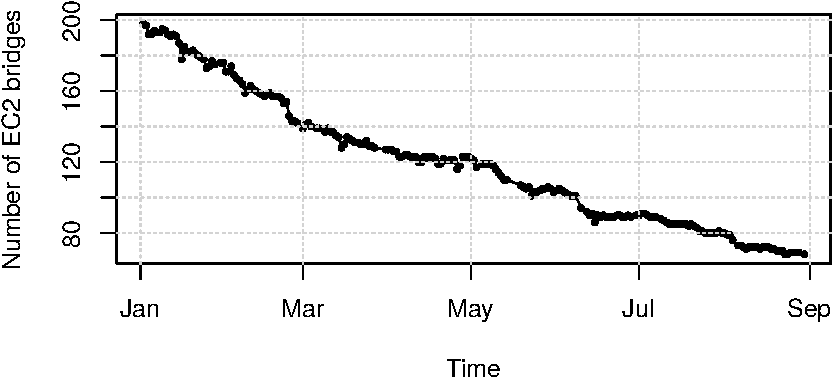
\includegraphics[width=\linewidth]{diagrams/torcloud.pdf}
	\caption{The amount of Tor Cloud~\cite{torcloud} bridges over time.  The
	numbers are steadily decreasing and the Tor Cloud system was discontinued in
	May 2015.}
	\label{fig:cloudbridges}
\end{figure}


\section{Conclusion}
\label{sec:conclusion}
In this paper, we worked towards finding and characterizing Sybils in the Tor
network.  We first invested significant engineering effort into the development
of sybilhunter, a command line tool to find and analyze Sybil groups.

Equipped with this new tool, we set out to analyze The Tor Project's network
data---archived as well as online data---for signs of Sybil relays.  We
uncovered several Sybil groups and gained new insight into real-world Sybil
attacks.  We found that 1) Sybil relays frequently look alike in their
appearance and behavior, 2) Sybil-running attackers differ greatly in their
technical sophistication, and 3) determining the root cause for Sybils is
challenging because it is often difficult to distinguish between benign and
malicious Sybils.

Given the lack of a central identity-verifying authority, it is always possible
for a well-executed Sybil attack to stay under our radar, but we found that a
simple set of tools and techniques can go a long way towards finding malicious
Sybils, thus making the Tor network more secure and trustworthy for its users.

Code, data, and other resources for our paper are available online at
\url{https://nymity.ch/sybilhunting/}.


% \section*{Acknowledgments}
We want to thank our shepherd, Tudor Dumitra\c{s}, for his guidance on improving
our work.  We also want to thank Georg Koppen, Prateek Mittal, Stefan Lindskog,
the Tor developers, and the wider Tor community for helpful feedback.  This
research was supported in part by the Center for Information Technology Policy
at Princeton University and by the National Science Foundation Awards
CNS-1540055 and CNS-1602399.


\bibliography{literature}{}
\bibliographystyle{unsrt}

\appendix

\section{Reproducing our work}
% \begin{lstlisting}
% go get git.torproject.org/user/phw/sybilhunter.git
% \end{lstlisting}
Redacted for anonymization.

\section{Mathematical metric}
\label{sec:metric}
The following conditions have to be met in order to classify as a mathematical
metric.  While points 1, 2, and 3 are typically straightforward to satisfy,
point 4, the triangle inequality, can turn out to be tricky.
\begin{enumerate}
	\item $d(x, y) \geq 0$
	\item $d(x, y) = 0$ iff $x = y$
	\item $d(x, y) = d(y, x)$
	\item $d(x, z) \leq d(x, y) + d(y, z)$
\end{enumerate}


\end{document}
